% Template for PLoS
% Version 3.4 January 2017
\documentclass[10pt,letterpaper]{article}
\usepackage[top=0.85in,left=2.75in,footskip=0.75in]{geometry}

% amsmath and amssymb packages, useful for mathematical formulas and symbols
\usepackage{amsmath,amssymb}

% Use adjustwidth environment to exceed column width (see example table in text)
\usepackage{changepage}

% Use Unicode characters when possible
\usepackage[utf8x]{inputenc}

% textcomp package and marvosym package for additional characters
\usepackage{textcomp,marvosym}

% cite package, to clean up citations in the main text. Do not remove.
% \usepackage{cite}

% Use nameref to cite supporting information files (see Supporting Information section for more info)
\usepackage{nameref,hyperref}

% line numbers
\usepackage[right]{lineno}

% ligatures disabled
\usepackage{microtype}
\DisableLigatures[f]{encoding = *, family = * }

% color can be used to apply background shading to table cells only
\usepackage[table]{xcolor}

% array package and thick rules for tables
\usepackage{array}

% create "+" rule type for thick vertical lines
\newcolumntype{+}{!{\vrule width 2pt}}

% create \thickcline for thick horizontal lines of variable length
\newlength\savedwidth
\newcommand\thickcline[1]{%
  \noalign{\global\savedwidth\arrayrulewidth\global\arrayrulewidth 2pt}%
  \cline{#1}%
  \noalign{\vskip\arrayrulewidth}%
  \noalign{\global\arrayrulewidth\savedwidth}%
}

% \thickhline command for thick horizontal lines that span the table
\newcommand\thickhline{\noalign{\global\savedwidth\arrayrulewidth\global\arrayrulewidth 2pt}%
\hline
\noalign{\global\arrayrulewidth\savedwidth}}


% Remove comment for double spacing
%\usepackage{setspace} 
%\doublespacing

% Text layout
\raggedright
\setlength{\parindent}{0.5cm}
\textwidth 5.25in 
\textheight 8.75in

% Bold the 'Figure #' in the caption and separate it from the title/caption with a period
% Captions will be left justified
\usepackage[aboveskip=1pt,labelfont=bf,labelsep=period,justification=raggedright,singlelinecheck=off]{caption}
\renewcommand{\figurename}{Fig}

% Use the PLoS provided BiBTeX style
% \bibliographystyle{plos2015}

% Remove brackets from numbering in List of References
\makeatletter
\renewcommand{\@biblabel}[1]{\quad#1.}
\makeatother

% Leave date blank
\date{}

% Header and Footer with logo
\usepackage{lastpage,fancyhdr,graphicx}
\usepackage{epstopdf}
\pagestyle{myheadings}
\pagestyle{fancy}
\fancyhf{}
\setlength{\headheight}{27.023pt}
\lhead{\includegraphics[width=2.0in]{PLOS-submission.eps}}
\rfoot{\thepage/\pageref{LastPage}}
\renewcommand{\footrule}{\hrule height 2pt \vspace{2mm}}
\fancyheadoffset[L]{2.25in}
\fancyfootoffset[L]{2.25in}
\lfoot{\sf PLOS}

%% Include all macros below
\newcommand{\lorem}{{\bf LOREM}}
\newcommand{\ipsum}{{\bf IPSUM}}

\usepackage{color}
\usepackage{fancyvrb}
\newcommand{\VerbBar}{|}
\newcommand{\VERB}{\Verb[commandchars=\\\{\}]}
\DefineVerbatimEnvironment{Highlighting}{Verbatim}{commandchars=\\\{\}}
% Add ',fontsize=\small' for more characters per line
\usepackage{framed}
\definecolor{shadecolor}{RGB}{248,248,248}
\newenvironment{Shaded}{\begin{snugshade}}{\end{snugshade}}
\newcommand{\AlertTok}[1]{\textcolor[rgb]{0.94,0.16,0.16}{#1}}
\newcommand{\AnnotationTok}[1]{\textcolor[rgb]{0.56,0.35,0.01}{\textbf{\textit{#1}}}}
\newcommand{\AttributeTok}[1]{\textcolor[rgb]{0.77,0.63,0.00}{#1}}
\newcommand{\BaseNTok}[1]{\textcolor[rgb]{0.00,0.00,0.81}{#1}}
\newcommand{\BuiltInTok}[1]{#1}
\newcommand{\CharTok}[1]{\textcolor[rgb]{0.31,0.60,0.02}{#1}}
\newcommand{\CommentTok}[1]{\textcolor[rgb]{0.56,0.35,0.01}{\textit{#1}}}
\newcommand{\CommentVarTok}[1]{\textcolor[rgb]{0.56,0.35,0.01}{\textbf{\textit{#1}}}}
\newcommand{\ConstantTok}[1]{\textcolor[rgb]{0.00,0.00,0.00}{#1}}
\newcommand{\ControlFlowTok}[1]{\textcolor[rgb]{0.13,0.29,0.53}{\textbf{#1}}}
\newcommand{\DataTypeTok}[1]{\textcolor[rgb]{0.13,0.29,0.53}{#1}}
\newcommand{\DecValTok}[1]{\textcolor[rgb]{0.00,0.00,0.81}{#1}}
\newcommand{\DocumentationTok}[1]{\textcolor[rgb]{0.56,0.35,0.01}{\textbf{\textit{#1}}}}
\newcommand{\ErrorTok}[1]{\textcolor[rgb]{0.64,0.00,0.00}{\textbf{#1}}}
\newcommand{\ExtensionTok}[1]{#1}
\newcommand{\FloatTok}[1]{\textcolor[rgb]{0.00,0.00,0.81}{#1}}
\newcommand{\FunctionTok}[1]{\textcolor[rgb]{0.00,0.00,0.00}{#1}}
\newcommand{\ImportTok}[1]{#1}
\newcommand{\InformationTok}[1]{\textcolor[rgb]{0.56,0.35,0.01}{\textbf{\textit{#1}}}}
\newcommand{\KeywordTok}[1]{\textcolor[rgb]{0.13,0.29,0.53}{\textbf{#1}}}
\newcommand{\NormalTok}[1]{#1}
\newcommand{\OperatorTok}[1]{\textcolor[rgb]{0.81,0.36,0.00}{\textbf{#1}}}
\newcommand{\OtherTok}[1]{\textcolor[rgb]{0.56,0.35,0.01}{#1}}
\newcommand{\PreprocessorTok}[1]{\textcolor[rgb]{0.56,0.35,0.01}{\textit{#1}}}
\newcommand{\RegionMarkerTok}[1]{#1}
\newcommand{\SpecialCharTok}[1]{\textcolor[rgb]{0.00,0.00,0.00}{#1}}
\newcommand{\SpecialStringTok}[1]{\textcolor[rgb]{0.31,0.60,0.02}{#1}}
\newcommand{\StringTok}[1]{\textcolor[rgb]{0.31,0.60,0.02}{#1}}
\newcommand{\VariableTok}[1]{\textcolor[rgb]{0.00,0.00,0.00}{#1}}
\newcommand{\VerbatimStringTok}[1]{\textcolor[rgb]{0.31,0.60,0.02}{#1}}
\newcommand{\WarningTok}[1]{\textcolor[rgb]{0.56,0.35,0.01}{\textbf{\textit{#1}}}}




\usepackage{forarray}
\usepackage{xstring}
\newcommand{\getIndex}[2]{
  \ForEach{,}{\IfEq{#1}{\thislevelitem}{\number\thislevelcount\ExitForEach}{}}{#2}
}

\setcounter{secnumdepth}{0}

\newcommand{\getAff}[1]{
  \getIndex{#1}{Monash University,Genentech}
}

\providecommand{\tightlist}{%
  \setlength{\itemsep}{0pt}\setlength{\parskip}{0pt}}

\begin{document}
\vspace*{0.2in}

% Title must be 250 characters or less.
\begin{flushleft}
{\Large
\textbf\newline{plyranges: a grammar for manipulating genomics data} % Please use "sentence case" for title and headings (capitalize only the first word in a title (or heading), the first word in a subtitle (or subheading), and any proper nouns).
}
\newline
\\
Stuart Lee\textsuperscript{\getAff{Monash University}},
Michael Lawrence\textsuperscript{\getAff{Genentech}},
Di Cook\textsuperscript{\getAff{Monash University}}\\
\bigskip
\textbf{\getAff{Monash University}}Department of Econometrics and Business Statistics, Clayton, Victoria,
Australia\\
\textbf{\getAff{Genentech}}Bioinformatics and Computational Biology, Genentech, Inc., South San
Francisco, California, United States of America\\
\bigskip
\end{flushleft}
% Please keep the abstract below 300 words
\section*{Abstract}
The Bioconductor project has created many powerful abstractions for
reasoning about genomics data, such as the \emph{Ranges} data structures
for representing genomic intervals. By recognising that these data
structures follow `tidy' data principles we have created a grammar of
genomic data manipulation that defines verbs for performing actions on
and between genomic interval data. This grammar simplifies performing
common genomic data analysis tasks via method chaining, type consistency
and results in creating human readable pipelines. We have implemented
this grammar as an Bioconductor/R package called plyranges.

% Please keep the Author Summary between 150 and 200 words
% Use first person. PLOS ONE authors please skip this step. 
% Author Summary not valid for PLOS ONE submissions.   

\linenumbers

% Use "Eq" instead of "Equation" for equation citations.
\hypertarget{introduction}{%
\section{Introduction}\label{introduction}}

Genomic data may be naturally represented as sets of pairs of integers
corresponding to the start and end points of sequences. Further
information such as strandedness and chromosome name may be added to
these sets to provide biological context. Because of the flexibility of
this representation supplemental information such as measurements
obtained from an experimental assay or annotations from a genome
database can be joined to their relevant sequences. In the
Bioconductor/R packages \texttt{IRanges} and \texttt{GenomicRanges}
these representations have been implemented as a suite of data
structures called \emph{Ranges} {[}1{]}. These data structures cover
many common data types encountered in bioinformatics analyses - a gene
can be represented with its coordinates, along with its identifier and
the identifiers of its exons; or an RNA-seq experiment may be
represented as sets of genes with a matching count column.

The Bioconductor infrastructure for computing with genomic ranges are
highly effecient and powerful, however the application programming
interface (API) for performing analysis tasks with \emph{Ranges} is
complex due to its large number of methods and classes. It also makes
resulting scripts written difficult for a non-programmer to read and
reason about. An alternative approach would be to implement a domain
specific language (DSL) as a fluent interface built on top
\emph{Ranges}. The goal of fluent interface is to enable users to write
human-readable code via method chaining and consistent function returns.
Fluent interfaces fit naturally in the context of Bioinformatics
workflows because they enable writing succinct pipelines.

Several other DSLs have been implemented to reason about genomics data.
Broadly, these are either implemented as query languages or as command
line tools embedded in the unix environment.\footnote{other ideas to
  mention GROK {[}2{]}} An example of the former is the Genome Query
Language (GQL) and its distributed implementation GenAp which use an
SQL-like syntax for fast retrieval of information from genomic databases
and BAM files {[}3{]}; {[}4{]}. Another example is the Genometric Query
Language (GMQL) which implements a relational algebra for combining big
genomic datasets {[}5{]}.\\
The command line application BEDtools develops an extensive algebra for
performing arithmetic between two or more sets of genomic regions
{[}6{]}. It also has a python interface which simplifies constructing
scripts for performing analyses based on BEDTools {[}7{]}.

The abstraction provided by the \emph{Ranges} data structures aligns
with the concept of tidy data {[}8{]}. The tidy data pattern is useful
because it allows us to see how the data relates to the design of an
experiment and the variables measured. Consequently, it makes both the
modelling and manipulation of data more systematic. The \emph{Ranges}
data structure follows this abstraction: it is a rectanglular table
corresponding to a single biological context. Each row contains a single
observation and each column a variable about that observation.

The tidy data abstraction has motivated the development of
\texttt{plyranges} a grammar of genomic data manipulation based on the
\emph{Ranges} data structures. It implements and extends the grammar
defined by the R package \texttt{dplyr} {[}9{]}. The grammar provides a
consistent way of interacting with and analysing genomic data via
methods for constructing, grouping, mutating, filtering, and summarising
\emph{Ranges} and an algebra for reasoning about actions on
\emph{Ranges} and relationships between \emph{Ranges}.

\hypertarget{design-and-implementation}{%
\section{Design and Implementation}\label{design-and-implementation}}

The \emph{plyranges} API implements a domain specific language using the
existing \emph{IRanges} and \emph{GenomicRanges} packages in
Bioconductor as a backend. Consequently, our API still has the speed and
effeciency of the aforementioned packages but with a more coherent
interface. The API also extends the grammar elements in \emph{dplyr} for
performing genomic specific manipulations such as finding overlapping
regions or nearest neighbour regions between many \emph{Ranges}. The
\emph{plyranges} API is specifically designed to enable fast interactive
analysis of \emph{Ranges} objects but can also be used for scripting
genomic data workflows.

We have desgined the API to be fluent. Every function call corresponds
to an action on a \emph{Ranges} object (they are named verbs) and where
possible functions have few arguments. Each verb is constructed to
enable a tab completion based workflow. Both of these aspects reduce the
cognitive load on a new user since most manipulations can be performed
with a vocabulary of several verbs, rather than having to memorise
functions with many arguments that are nouns (as is required in the
existing Bioconductor packages). This is also has the advantage of
allowing users to write human readable code because verbs describe what
the code is doing rather than how its doing it.

Workflows can be composed by chaining verbs together via the pipe
operator,\texttt{\%\textgreater{}\%} (exported from the R package
\emph{magrittr}). This is possible because every function call is
endomorphic: when the input is \emph{Ranges} object the output will also
be a \emph{Ranges} object. One advantage of this static typing is that
it does not require any additional learning of classes beyond
\emph{Ranges} and the \emph{DataFrame} classes. This is similar to the
bedtools API, where the output is usually a BED file. However, it
strongly deviates from the design of the \emph{Ranges} Bioconductor
packages, where many methods return a new class upon return. The
Bioconductor design enables effecient computing as users are exposed to
low-level features of its API which \emph{plyranges} trys to abstract
away. Method chaining via the pipe operator can also be difficult to
debug, as there multiple points of failure.

In order to provide a compatible API with \emph{dplyr}, \emph{plyranges}
makes extensive use of non-standard evaluation in R via the \emph{rlang}
package. Simply, this means that compuations are performed and evaluated
in the context of the Ranges objects, which emphasises the interactive
nature of the API. This has the disadvantage that programming with
\emph{plyranges} becomes more difficult because a user needs to capture
expressions inside function calls and then unquote them.

\hypertarget{working-with-ranges}{%
\subsection{Working with Ranges}\label{working-with-ranges}}

\hypertarget{construction-and-importoutput}{%
\subsubsection{Construction and
Import/Output}\label{construction-and-importoutput}}

The \emph{plyranges} API provides the methods \texttt{as\_granges()} and
\texttt{as\_iranges()} for constructing Ranges from tabular data
structures, such as the \emph{data.frame} in base R. These methods use
non-standard evaluation so columns in a \emph{data.frame} can be
modified before a \emph{Ranges} object is created. The API also has
convienence methods for annotating or extracting annotations from
Genomic Ranges objects with the \texttt{set\_genome\_info()} and
\texttt{get\_genome\_info()} functions.

There is a consistent framework for reading and writing files from and
to common genomic data formats, using the \texttt{rtracklayer} package
as a backend. The methods are implemented in the \texttt{read\_/write\_}
family of functions, currently \emph{plyranges} can read and write BAM,
BED, BEDPE, narrowPeaks, GFF/GTF, WIG and BigWig files.

As an example, we use the Bioconductor package AnnotationHub to search
for BigWig files from ChIP-Seq experiments from the Human Epigenome
Roadmap project. We choose to focus on assays for primary T CD8+ memory
cells from peripheral blood. We can then read the BigWig file
corresponding to the H3 lysine 27 trimethylation (H3K27Me3) methylation
mark over chromosome 10. First we gather the BigWig file and extract its
annotation information and filter it to chromosome 10.

\begin{Shaded}
\begin{Highlighting}[]
\CommentTok{# E048 corresponds to CD8+ T cells from peripheral blood}
\KeywordTok{library}\NormalTok{(plyranges)}
\KeywordTok{library}\NormalTok{(AnnotationHub)}
\NormalTok{q <-}\KeywordTok{query}\NormalTok{(}\KeywordTok{AnnotationHub}\NormalTok{(), }\KeywordTok{c}\NormalTok{(}\StringTok{"EpigenomeRoadMap"}\NormalTok{, }\StringTok{"E048"}\NormalTok{))}

\NormalTok{bw_file <-}\StringTok{ }\NormalTok{q[[}\StringTok{"AH33458"}\NormalTok{]] }

\NormalTok{chr10_ranges <-}\StringTok{ }\NormalTok{bw_file }\OperatorTok\StringTok{ }
\StringTok{  }\KeywordTok{get_genome_info}\NormalTok{() }\OperatorTok
\StringTok{  }\KeywordTok{filter}\NormalTok{(seqnames }\OperatorTok{==}\StringTok{ "chr10"}\NormalTok{)}
\end{Highlighting}
\end{Shaded}

Then we read the BigWig file only extracting scores if they overlap
chromosome 10. We then add annotation information to ensure we know we
are working with the hg19 genome build.

\begin{Shaded}
\begin{Highlighting}[]
\NormalTok{chr10_scores <-}\StringTok{ }\NormalTok{bw_file }\OperatorTok
\StringTok{  }\KeywordTok{read_bigwig}\NormalTok{(}\DataTypeTok{overlap_ranges =}\NormalTok{ chr10_ranges) }\OperatorTok
\StringTok{  }\KeywordTok{set_genome_info}\NormalTok{(}\DataTypeTok{genome =} \StringTok{"hg19"}\NormalTok{)}
\NormalTok{chr10_scores}
\end{Highlighting}
\end{Shaded}

\begin{verbatim}
#> GRanges object with 5789841 ranges and 1 metadata column:
#>             seqnames                 ranges strand |              score
#>                <Rle>              <IRanges>  <Rle> |          <numeric>
#>         [1]    chr10         [    1, 60602]      * | 0.0422799997031689
#>         [2]    chr10         [60603, 60781]      * |  0.163240000605583
#>         [3]    chr10         [60782, 60816]      * |  0.372139990329742
#>         [4]    chr10         [60817, 60995]      * |  0.163240000605583
#>         [5]    chr10         [60996, 61625]      * | 0.0422799997031689
#>         ...      ...                    ...    ... .                ...
#>   [5789837]    chr10 [135524723, 135524734]      * |  0.144319996237755
#>   [5789838]    chr10 [135524735, 135524775]      * |  0.250230014324188
#>   [5789839]    chr10 [135524776, 135524784]      * |  0.427789986133575
#>   [5789840]    chr10 [135524785, 135524806]      * |  0.730019986629486
#>   [5789841]    chr10 [135524807, 135524837]      * |   1.03103005886078
#>   -------
#>   seqinfo: 25 sequences from hg19 genome
\end{verbatim}

\hypertarget{manipulation-of-ranges}{%
\subsubsection{Manipulation of Ranges}\label{manipulation-of-ranges}}

The \emph{plyranges} API exports the six core verbs from the
\emph{dplyr} package and modifys them for use with simple \emph{Ranges}
and \emph{Genomic Ranges}. The verb \texttt{mutate()} takes a Ranges
object and a set of name-value pairs and generates a new Ranges object
that with modified or new metadata columns or modified core components
(start, end, width, seqnames, strand). The use of \texttt{mutate()}
means that a user no longer needs knowledge of the accessors of the
Ranges object, as they can modify them in place. The \texttt{filter()}
function takes a Ranges object and logical expressions and restricts
Ranges object to where the logical expression evaluates to true. The
\texttt{summarise()} function takes a Ranges object and a set of
name-value pairs and aggregates the Ranges according to functions
evaluated in the name-value pairs. As \texttt{summarise()} is an
aggregation it may break the structure of the of a Ranges object, hence
it returns a DataFrame object. The \texttt{select()} function determines
which metadata columns are returned and the order they are returned in.
The \texttt{arrange()} function sorts a Ranges object by named
variables. The \texttt{group\_by()} function creates an implicit
grouping of Ranges object according to variables in the Ranges object.
This modifies the actions of \texttt{mutate()}, \texttt{summarise()} and
\texttt{filter()}, so they are performed on each partition created by
the grouping. The \texttt{group\_by()} operation acts as a replacement
for the \emph{GenomicRangesList} class in the original
\emph{GenomicRanges} API.

The \emph{plyranges} API introduces additional summary verbs,
\texttt{reduce\_ranges()} and \texttt{disjoin\_ranges()}that return
Ranges objects after being returned. The \texttt{reduce\_ranges()}
operation merges overlapping and neighbour ranges, while
\texttt{disjoin\_ranges()} expands ranges by taking the union of end
points.

The \texttt{reduce\_ranges()} operation could be used to find coverage
peaks accross chromosome 10. We can manually set a threshold to restrict
genomic regions to have a coverage score of greater than 8, and then
merge those regions and compute the maximum coverage over all the
regions that were reduced.

\begin{Shaded}
\begin{Highlighting}[]
\NormalTok{all_peaks <-}\StringTok{ }\NormalTok{chr10_scores }\OperatorTok\StringTok{ }
\StringTok{  }\KeywordTok{filter}\NormalTok{(score }\OperatorTok{>}\StringTok{ }\DecValTok{8}\NormalTok{) }\OperatorTok\StringTok{ }
\StringTok{  }\KeywordTok{reduce_ranges}\NormalTok{(}\DataTypeTok{score =} \KeywordTok{max}\NormalTok{(score))}
\end{Highlighting}
\end{Shaded}

The combination of these verbs together encapsulate most operations that
can be performed in the original \emph{IRanges} and \emph{GenomicRanges}
packages without the user be exposed to new classes. In those packages
to perform the above operation requires users to understand what an run
length encoding object and views object means and perform additional
manipulations to return the result back to a \emph{Ranges}.

\hypertarget{arithimetic-on-ranges}{%
\subsubsection{Arithimetic on Ranges}\label{arithimetic-on-ranges}}

The API has an expressive algebra for performing arithmetic on Ranges
via the verbs \texttt{set\_width()} and \texttt{stretch()}. As the names
suggest \texttt{set\_width()} modifies the width of a Ranges object,
while \texttt{stretch} extends the start and end of a Ranges object.
These can be chained with the anchoring functions
\texttt{anchor\_start()}, \texttt{anchor\_end()},
\texttt{anchor\_center()}, \texttt{anchor\_3p()} or
\texttt{anchor\_5p()}, which fix the coordinates of a Ranges object in
place. Moreover, the \texttt{shift\_} and \texttt{flank\_} family of
functions can be used to shift all coordinates in a Ranges object or
generate flanking regions from a Ranges object to the left, right,
upstream or downstream of the input. Unlike, the Bioconductor API,
\emph{plyranges} makes it expclit via function calls whether to take
into account the strand information of a \emph{Ranges} object.

Returning to the Ranges object containing normalised coverage scores for
the methylation data, we can filter to find the coordinates of the peak
containing maximum coverage score. We can then find a 5000 nt region
centered around the maximum position by anchoring and modifying the the
width.

\begin{Shaded}
\begin{Highlighting}[]
\NormalTok{chr10_max_score_region <-}\StringTok{ }\NormalTok{chr10_scores }\OperatorTok
\StringTok{  }\KeywordTok{filter}\NormalTok{(score }\OperatorTok{==}\StringTok{ }\KeywordTok{max}\NormalTok{(score)) }\OperatorTok\StringTok{ }
\StringTok{  }\KeywordTok{anchor_center}\NormalTok{() }\OperatorTok
\StringTok{  }\KeywordTok{set_width}\NormalTok{(}\DecValTok{5000}\NormalTok{)}
\end{Highlighting}
\end{Shaded}

\hypertarget{overlapping-ranges}{%
\subsubsection{Overlapping Ranges}\label{overlapping-ranges}}

A common operation to perform between two \emph{Ranges} objects is to
find overlaps or nearest neighbours. The \emph{plyranges} API recasts
these operations as `joins' or `pairing' operations. For overlaps, there
are three join operations: \texttt{join\_overlap\_intersect()},
\texttt{join\_overlap\_inner()} and \texttt{join\_overlap\_left()} which
are shown in figure (\ref{fig:olap}).

\begin{figure}

{\centering \includegraphics{paper_files/figure-latex/olap-1} 

}

\caption{The three overlap joins: the query and subject ranges are coloured by their metadata. When an overlap is performed the resulting range is filled by the query metadata and the metadata from the subject colours the outside of the range.}\label{fig:olap}
\end{figure}

These operations consider any overlap between two input ranges and
return any corresponding metadata from both Ranges objects as metadata.
The intersect join takes the intersect of the start and end coordinates
of overlapping intervals of the query and subject Ranges (for
GenomicRanges it also accounts for sequence name), when there is a
overlap the metadata corresponding to the query and subject Ranges are
returned. Similarly, inner join takes the start and end coordinates of
the query Ranges that overlap the subject Ranges and returns metadata of
the overlapping query and subject Ranges. Finally, the left join
performs a left outer join between the query and subject Ranges, it
returns all genomic intervals from the query ranges, and returns missing
values in metadata columns when there is no overlap.

The overlap innner join could be used to restrict the chromosome 10
normalised coverage scores that are within the 5000nt region that
contains the max peak on chromosome 10 (visualised in figure
\ref{fig:peak-viz}).

\begin{Shaded}
\begin{Highlighting}[]
\NormalTok{peak_region <-}\StringTok{ }\NormalTok{chr10_scores }\OperatorTok
\StringTok{  }\KeywordTok{join_overlap_inner}\NormalTok{(., }
\NormalTok{                     chr10_max_score_region }\OperatorTok\StringTok{ }
\StringTok{                       }\KeywordTok{select}\NormalTok{(}\OperatorTok{-}\NormalTok{score))}
\end{Highlighting}
\end{Shaded}

\begin{figure}

{\centering 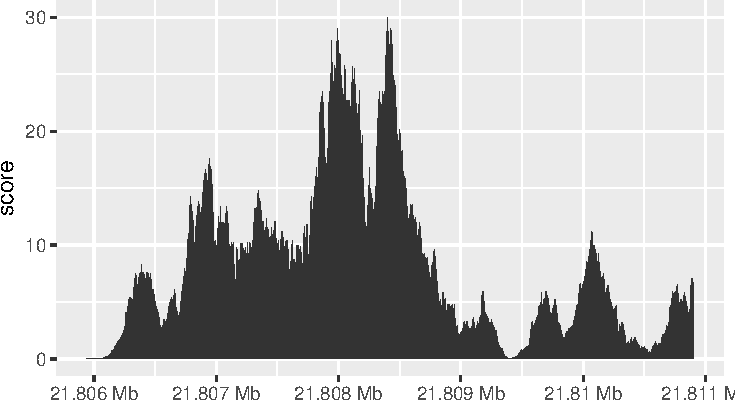
\includegraphics{paper_files/figure-latex/peak-viz-1} 

}

\caption{Visualisation of normalised coverage scores accross a 5000nt region of chromosome 10 from H3K27Me3 ChIP-Seq assay from the Human Epigenome Roadmap project.}\label{fig:peak-viz}
\end{figure}

A user may also restrict or group by overlaps with the
\texttt{filter\_by\_overlaps()}, \texttt{filter\_by\_non\_overlaps()}
and \texttt{group\_by\_overlaps()}. All overlap methods can be modified
with the \texttt{within} suffix (which changes the type of overlap from
`any' to `within') or the \texttt{directed} suffix (which takes into
account the strand of a GenomicRanges object.).

For nearest neighbours, the \texttt{plyranges} API provides
\texttt{join\_nearest()}, \texttt{join\_precede()}, and
\texttt{join\_follow()} functions. These functions are similar to the
overlapping functions, in that they return the query ranges that are
nearest (or precede or follow) the subject ranges and add metadata from
the subject ranges when the query is a nearest neighbour of the subject.
Like the overlap joins, these functions can modified with suffixes to
find nearest neighbours that are left, right, upstream or downstream of
the subject.

The pairing operations, \texttt{pair\_overlap()},
\texttt{pair\_nearest()}, \texttt{pair\_follow()}, and
\texttt{pair\_precede()} are similar to the join operation but instead
of returning a Ranges, they pair up the subject and query Ranges objects
into a DataFrame, alongside their metadata columns. This data structure
is similar to the \emph{Pairs} data structure in the \emph{S4Vectors}
package or the BED-PE file format.

\hypertarget{results}{%
\section{Results}\label{results}}

\begin{itemize}
\tightlist
\item
  Redo an analysis in https://www.nature.com/articles/nature14248
\end{itemize}

\hypertarget{availablilty-and-future-work}{%
\section{Availablilty and Future
Work}\label{availablilty-and-future-work}}

The \emph{plyranges} package is avaiable on the Bioconductor project
website \url{https://bioconductor.org} or can be accessed via Github
\url{https://github.com/sa-lee/plyranges}. We aim to continue developing
the \texttt{plyranges} package and extend it for use with more complex
data structures such as the \emph{SummarizedExperiment} class, which can
be used for analysing transcriptomic and variant data. As the
\texttt{plyranges} interface encourages tidy data practices it
integrates well with the principles of the grammar of graphics, we aim
to use it for the visualisation of multimodal biological datasets.

\hypertarget{references}{%
\section*{References}\label{references}}
\addcontentsline{toc}{section}{References}

\hypertarget{refs}{}
\leavevmode\hypertarget{ref-Lawrence2013-wg}{}%
1. Lawrence M, Huber W, Pagès H, Aboyoun P, Carlson M, Gentleman R, et
al. Software for computing and annotating genomic ranges. PLoS Comput
Biol. 2013;9.
doi:\href{https://doi.org/10.1371/journal.pcbi.1003118}{10.1371/journal.pcbi.1003118}

\leavevmode\hypertarget{ref-Ovaska2013-gd}{}%
2. Ovaska K, Lyly L, Sahu B, Jänne OA, Hautaniemi S. Genomic region
operation kit for flexible processing of deep sequencing data. IEEE/ACM
Trans Comput Biol Bioinform. 2013;10: 200--206.
doi:\href{https://doi.org/10.1109/TCBB.2012.170}{10.1109/TCBB.2012.170}

\leavevmode\hypertarget{ref-Kozanitis2014-va}{}%
3. Kozanitis C, Heiberg A, Varghese G, Bafna V. Using genome query
language to uncover genetic variation. Bioinformatics. 2014;30: 1--8.
doi:\href{https://doi.org/10.1093/bioinformatics/btt250}{10.1093/bioinformatics/btt250}

\leavevmode\hypertarget{ref-Kozanitis2016-bm}{}%
4. Kozanitis C, Patterson DA. GenAp: A distributed SQL interface for
genomic data. BMC Bioinformatics. 2016;17: 63.
doi:\href{https://doi.org/10.1186/s12859-016-0904-1}{10.1186/s12859-016-0904-1}

\leavevmode\hypertarget{ref-Kaitoua2017-pw}{}%
5. Kaitoua A, Pinoli P, Bertoni M, Ceri S. Framework for supporting
genomic operations. IEEE Trans Comput. 2017;66: 443--457.
doi:\href{https://doi.org/10.1109/TC.2016.2603980}{10.1109/TC.2016.2603980}

\leavevmode\hypertarget{ref-Quinlan2010-gc}{}%
6. Quinlan AR, Hall IM. BEDTools: A flexible suite of utilities for
comparing genomic features. Bioinformatics. 2010;26: 841--842.
doi:\href{https://doi.org/10.1093/bioinformatics/btq033}{10.1093/bioinformatics/btq033}

\leavevmode\hypertarget{ref-Dale2011-js}{}%
7. Dale RK, Pedersen BS, Quinlan AR. Pybedtools: A flexible python
library for manipulating genomic datasets and annotations.
Bioinformatics. 2011;27: 3423--3424.
doi:\href{https://doi.org/10.1093/bioinformatics/btr539}{10.1093/bioinformatics/btr539}

\leavevmode\hypertarget{ref-Wickham2014-jc}{}%
8. Wickham H. Tidy data. Journal of Statistical Software, Articles.
2014;59: 1--23.
doi:\href{https://doi.org/10.18637/jss.v059.i10}{10.18637/jss.v059.i10}

\leavevmode\hypertarget{ref-Wickham2017-dplyr}{}%
9. Wickham H, Francois R, Henry L, Müller K. Dplyr: A grammar of data
manipulation {[}Internet{]}. 2017. Available:
\url{https://CRAN.R-project.org/package=dplyr}

\nolinenumbers


\end{document}

